% 	TEMPLATE DE RELACIÓN DE EJERCICIOS
%
% Creador: Juamagdev

% ------------------------------------------------------------------
% ---------------------- Package imports ---------------------------
% ------------------------------------------------------------------
\documentclass[11pt, a4paper]{exam}
\usepackage[utf8]{inputenc}		% UTF-8
\usepackage[spanish]{babel}		% Idioma
\usepackage{graphicx}			% Para importar gráficos
\usepackage{amsthm, amsfonts, amssymb, amssymb} % Todos los paquetes AMS
\usepackage{mathtools}          % Arregla bugs de AMS
\usepackage{hyperref}			% Para \href{URL}{text}
\usepackage{enumitem}			% Para enumerar
\usepackage{color} 				% Para definir colores nuevos
\usepackage{lastpage}			% Para \pageref{LastPage}
\usepackage{booktabs}					% Tablas profesionales
\usepackage{parskip}					% Espacio de párrafos
\usepackage[sharp]{easylist}			% Para litas
\usepackage[expansion=false]{microtype} % Soluciona bugs de tipografias
\usepackage[margin=2.25cm, includehead, includefoot]{geometry}
\usepackage{cancel}
\usepackage{pgfplots}
\usepackage{listings}



% ------------------------------------------------------------------
% ---------------------- Constantes --------------------------------
% ------------------------------------------------------------------
% Las constantes mas importantes
\newcommand{\mytitle}{Ejercicio Máquina de Turing M4}
\newcommand{\mysubject}{Algoritmia y Complejidad}
\newcommand{\mydate}{\today}
\newcommand{\myauthor}{Juan Manuel García Delgado}

% Redefinir para cada caso
\newcommand{\myrhead}{Universidad de Málaga}
\newcommand{\mypagename}{Página}
\newcommand{\mycreated}{Creado por: }
\newcommand{\mysolname}{Solución}
\renewcommand{\solutiontitle}{\noindent\textbf{\mysolname.}\hspace{0.75em}}
\pointpoints{point}{points}

\providecommand{\abs}[1]{\lvert#1\rvert}

% ------------------------------------------------------------------
% ---------------------- Ajustes -----------------------------------
% ------------------------------------------------------------------
% \shadedsolutions
\printanswers % Alternative: \noprintanswers, \printanswers
%\rhead{{\scshape {\footnotesize  \myrhead}}}
%\cfoot{\mypagename \enspace \thepage}
\definecolor{SolutionColor}{rgb}{0.8,0.9,1} % light blue

% Cabeceras y pie de página
\runningfootrule
\firstpagefootrule
\firstpagefooter{\mysubject}{}{\mypagename\ \thepage\ de \pageref*{LastPage}}
\runningfooter{\mysubject}{}{\mypagename\ \thepage\ de \pageref*{LastPage}}
\runningheader{}{}{
\includegraphics[width = 3 cm]{figs/logo.pdf}}
\firstpageheadrule
\firstpageheader{\mydate}{\mytitle}{\pageref*{LastPage} páginas en total}

% Answer command for double lines
\def\answer#1{\underline{\underline{#1}}}

% ------------------------------------------------------------------
% ---------------------- Documento ---------------------------------
% ------------------------------------------------------------------
\begin{document}
\pagestyle{headandfoot}
\noindent {\scshape \Large  \mytitle
    \ifprintanswers
        \enspace (\mysolname	 )
    \fi
} \\
\noindent {\mycreated \enspace  \myauthor} \vspace{1em}
\hrule \hrule
\vspace{5mm}

% ------------------------------------------------------------------
% ---------------------- Contenido ---------------------------------
% ------------------------------------------------------------------

\begin{questions}
    \addpoints
    \question {\bfseries Crea las maquinas de turing para el siguiente lenguaje en su versión multicinta y unicinta:}
    \begin{equation*}
        L = \left\lbrace \#x_1\#x_2\#...\#x_l | x_i \in \left\lbrace 0, 1 \right\rbrace^*, x_i \neq x_j, i\neq j \right\rbrace
    \end{equation*}
    
    \begin{parts}
        \part Multicinta
        \begin{solution}
            \\
            % Una máquina de Turing multicinta es una variante de la máquina de Turing. Es un modelo matemático abstracto de un dispositivo que puede realizar cómputos. A diferencia de la máquina de Turing clásica, que tiene una sola cinta de entrada/salida, la máquina de Turing multicinta tiene varias cintas. En cada cinta, se puede leer y escribir información de entrada y salida.
            El lenguaje que nuestra maquina de tuirng que debe reconocer es el de un conjunto finito de palabras formadas por 0s o por 1s, separadas por el simbolo $\#$, con la caracterísitca de que no se puede repetir ninguna palabra entre cada $\#$. Es el llamado problema de los elementos distintos.
            \\
            \\
            Es decir, cadenas formadas por 0s y 1s, separadas por $\#$, siempre que no se repitan estas cadenas. Por ejemplo:
            \begin{enumerate}
                \item La cadena $\#100\#11\#101\#00$ es válida.
                \item La cadena $\#000\#10\#111\#000$ no es válida.
                \item La cadena $\#010\#10\#10\#00$ no es válida.
                \item La cadena $\#010\#1011\#01\#0$ es válida.
            \end{enumerate}

            La maquina de turing tendrá 2 cintas, en la primera de ellas se pondra la cadena para ser reconocida, en la segunda es donde se combrobara que no hay cadenas. Para ello la maquina realiza los siguientes pasos:
            \begin{enumerate}
                \item La maquina copia el separador $\#$ en la segunda cinta y la primera palabra, y los elimina de la primera cinta. Este separador para alinear cada separador y poder comparar digito por digito.
                \item Ahora la maquina alinea los separadores de ambas cintas.
                \item A continuación la maquina comprueba simbolo por símbolo que no se repiten. En caso de que encuentre un simbolo que sea distinto, ya no es necesario que compruebe y se dirige al proximo separador. Si todos los simbolos son iguales y no encuentra uno distinto, al llegar al separador rechaza la cadena.
                \item Se ejecutan las pasos 2 y 3 hasta llegar al final (un espacio en blanco).
                \item Al llegar al final, se vuelve al principio y se ejecutan la secuencia de nuevo desde el paso 1.
            \end{enumerate}
            En caso de que la maquina rechace la cadena, se parara mostrando de forma alineado el primer elemento que ha encontrado repetido.
            \\
            \\
            La maquina aceptará la cadena cuando en la primera cinta no haya simbolos. En cualquier otro caso, la cadena sera rechazada.
            A continuación se muestra el autómata que define la máquina de Turing. 
            \\
            \\
            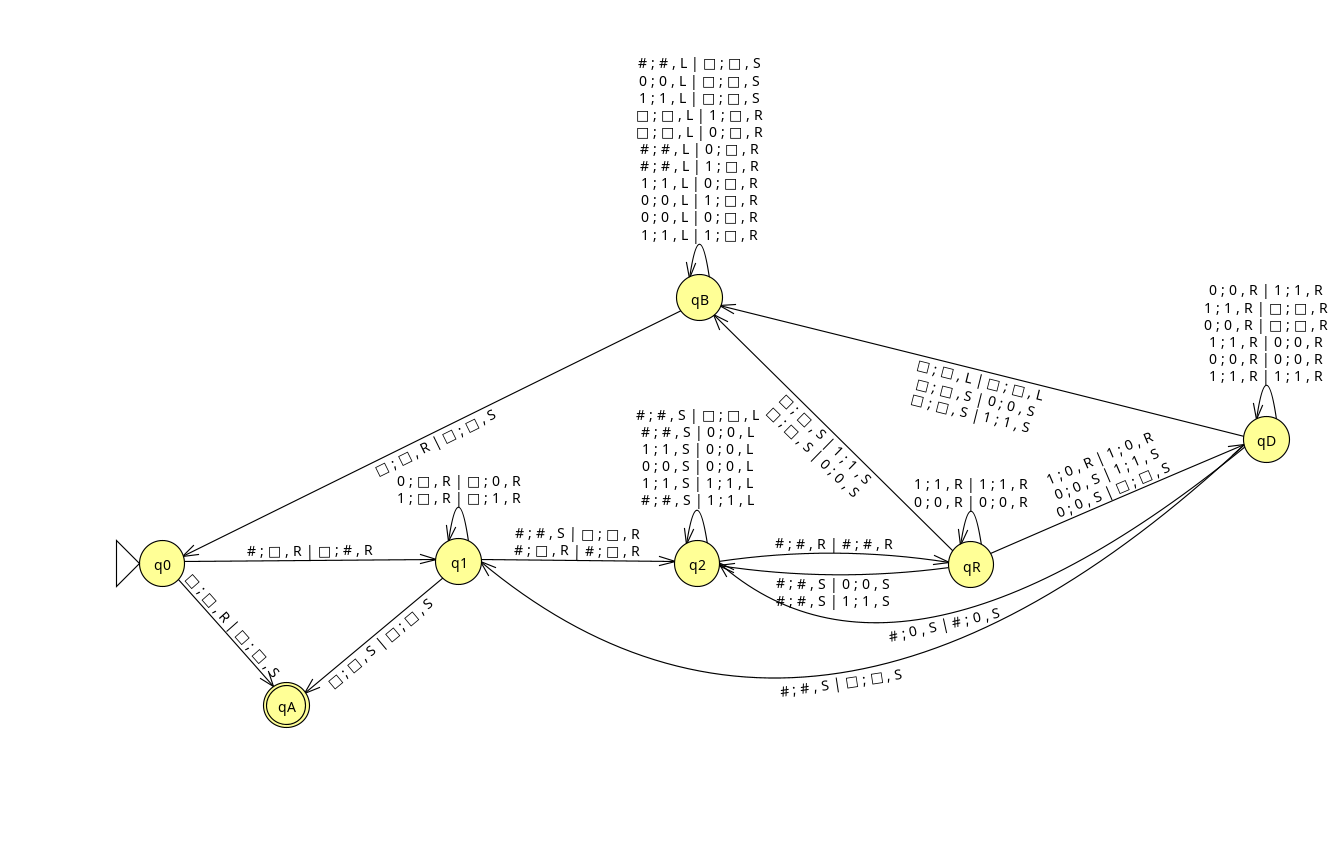
\includegraphics[width = 14 cm]{figs/M4Multicinta.png}
            \\Puede probar la maquina de turing en el siguiente simulador, donde ya se encuentra cargada la máquina de Turing: \url{http://turingmachinesimulator.com/shared/atughrsuvx}
            \\
            \\
            También puede encontrar todo el codigo de la máquina usada en el simulador, con los estados y transiciones en el repositorio de github, junto con el autómata generado por JFLAP, dentro de la carpeta de utilities: 
        \end{solution}

        \part Unicinta

        \begin{solution}
        \end{solution}
    \end{parts}

\end{questions}



%\hrule
%\subsection*{For retting}
%Ikke skriv noe her. \par \noindent
%\gradetable[h][questions]	
\end{document}